% Created 2021-12-08 Wed 09:53
% Intended LaTeX compiler: pdflatex
\documentclass[10pt]{beamer}
\usepackage[utf8]{inputenc}
\usepackage[T1]{fontenc}
\usepackage{graphicx}
\usepackage{grffile}
\usepackage{longtable}
\usepackage{wrapfig}
\usepackage{rotating}
\usepackage[normalem]{ulem}
\usepackage{amsmath}
\usepackage{textcomp}
\usepackage{amssymb}
\usepackage{capt-of}
\usepackage{hyperref}
\usepackage{physics}
\usetheme{default}
\author{S Shri Hari}
\date{\today}
\title{Simulating Active Dumbbells using Langevin Dynamics}
\hypersetup{
 pdfauthor={S Shri Hari},
 pdftitle={Simulating Active Dumbbells using Langevin Dynamics},
 pdfkeywords={},
 pdfsubject={},
 pdfcreator={Emacs 27.2 (Org mode 9.4.5)}, 
 pdflang={English}}
\begin{document}

\maketitle




\begin{frame}[label={sec:orgbab2fe4}]{Active Matter: Introduction}
\begin{block}{Definition:}
\begin{itemize}
\item Aggregate of units that consume energy to move / exert mechanical forces.
\end{itemize}
\end{block}
\begin{block}{Examples:}
\begin{itemize}
\item Bacterial Colonies
\item Self Assembling biomolecules
\item School of Fish, Flock of Birds
\end{itemize}
\end{block}
\begin{block}{Key Features:}
\begin{itemize}
\item Non-trivial behaviour exhibited when in large numbers / densities
\item Example: Self-Organization, Phase Separation, etc.
\end{itemize}
\end{block}
\end{frame}

\begin{frame}[label={sec:orgff9ddea}]{Active Matter: Example 1}
\begin{figure}[htbp]
\centering
\includegraphics[width=.9\linewidth]{./ExAct1.png}
\captionof{figure}{Internal Flow observed in high-density phases of active swimmers}
\end{figure}

\href{https://www.youtube.com/watch?v=j6dBq0F12nY}{Video Demonstrating Internal Flow Structure of Swimmers at high local concentrations}
\end{frame}

\begin{frame}[label={sec:orgd84b9b8}]{Active Matter: Example 2}
\begin{figure}[htbp]
\centering
\includegraphics[width=7cm]{./Boids.png}
\captionof{figure}{Boids is an artificial life program, developed by Craig Reynolds in 1986, which simulates the flocking behaviour of birds. The name "boid" corresponds to a shortened version of "bird-oid object", which refers to a bird-like object.}
\end{figure}

Credits: \href{https://www.labri.fr/perso/nrougier/from-python-to-numpy/#spatial-vectorization}{'From Python to NumPy' by Nicolas P. Rougier}

\href{./Boids.mp4}{Link to Video}
\end{frame}

\begin{frame}[label={sec:org8dbd5f6}]{Motivation}
\begin{block}{The Experiment:}
\begin{itemize}
\item "Cooperation in a fluid swarm of fuel-free micro-swimmers" by MYB Zion, A Modin, Y Caba, PM Chaikin (2021). \href{https://arxiv.org/abs/2012.15087}{arXiv: 2012.15087}
\end{itemize}
\end{block}
\begin{block}{Key Features}
\begin{itemize}
\item Constructed particles that are active but 'fuel-free'. Dynamics of Particles unaffected by local fuel concentrations.
\item Study focused on behaviour exhibited by aggregates
\begin{itemize}
\item Homogeneous system of Active Particles
\item Heterogenous system: Mixture of Active and Passive
\end{itemize}
\item Homogeneous System: Motility Induced Phase Separation (MIPS)
\item Heterogeneous System: A new phase - 'Corralling'; Passive Particles compressed to HCP by active particles
\end{itemize}
\end{block}
\end{frame}

\begin{frame}[label={sec:org969b0a9}]{}
\begin{center}
\includegraphics[width=.9\linewidth]{./Chaikin.png}
\end{center}
\end{frame}

\begin{frame}[label={sec:orgb312622}]{The Experiment: Key Details}
\begin{block}{Particles:}
\begin{itemize}
\item Passive: Spherical liquid droplets of n-dodecane in oil-water emulsion
\item Active: Light Absorbing Particle coupled to passive sphere; 'Peanut' Shaped
\item Medium: Water; Particles exhibit Brownian Motion
\end{itemize}
\end{block}
\begin{block}{Activity}
\begin{itemize}
\item Energy for active particles derived from light
\item Temperature gradient formed by light absorbing particles heating water surrounding it when exposed to light; Gradient verly localized to the particle
\item Propulsion along the axis due to thermo-capillary effect
\item Continuous relation between flux and activity
\end{itemize}
\end{block}
\end{frame}

\begin{frame}[label={sec:org15c105f}]{Relevant Study: Active Dumbbells}
\begin{itemize}
\item "Dynamics of a homogeneous active dumbbell system" by A Suma, G Gonnella, G Laghezza, A Lamura, A Mossa… - Physical Review E, 2014. \href{https://journals.aps.org/pre/abstract/10.1103/PhysRevE.90.052130}{Phys. Rev. E 90, 052130}
\item A Theoretical + Computational study about the system of active dumbbells
\item Behaviour observed similar to previous experiment's study on Homogeneous System
\end{itemize}
\end{frame}

\begin{frame}[label={sec:orgc172cf9}]{Simulating the System}
\begin{itemize}
\item Need to write own code from scratch to implement the driving forces
\item Reason: Lack of support to assign forces dynamically to each particle in LAMMPS
\item Objective of the Project: To simulate the heterogeneous system and observe/study the 'coralling' phase
\end{itemize}
\end{frame}

\begin{frame}[label={sec:org4a011f7}]{The Model: Potentials}
\begin{itemize}
\item Weeks-Chandler-Anderson(WCA) Potential
\end{itemize}
\begin{equation}
V_{WCA}(r) = \begin{cases}
V_{LJ}(r) - V_{LJ}(r_c) & r < r_c\\
0 & r > r_c
\end{cases}
\end{equation}
\begin{equation}
V_{LJ} = 4\epsilon\bqty{\pqty{\frac{\sigma}{r}}^{12} - \pqty{\frac{\sigma}{r}}^{6}} \ \ ;\ \ r_c = 2^{1/6}\sigma
\end{equation}
where \(\sigma\) is the diameter of the spherical particles

\begin{itemize}
\item Spring: Finite Extensible Nonlinear Elastic (FENE)
\end{itemize}
\begin{equation}
F_{FENE}(\mathbf{r}) = \frac{- k \mathbf{r}}{1 - \pqty{r / r_0}^2}
\end{equation}
where \(r_0\) represents the maximum spring length
\end{frame}

\begin{frame}[label={sec:org273ed34}]{Plot: Potentials}
\begin{center}
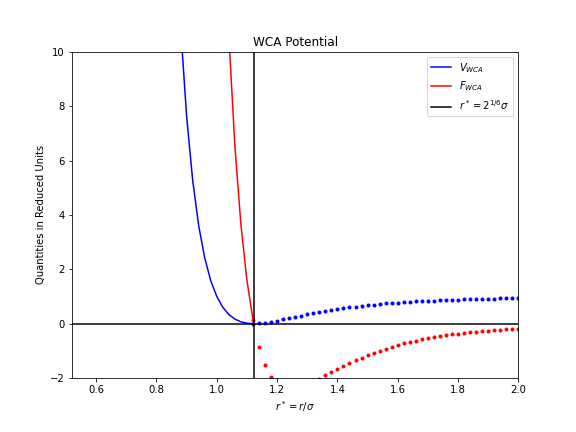
\includegraphics[height=4cm\textwidth]{./WCA.png}
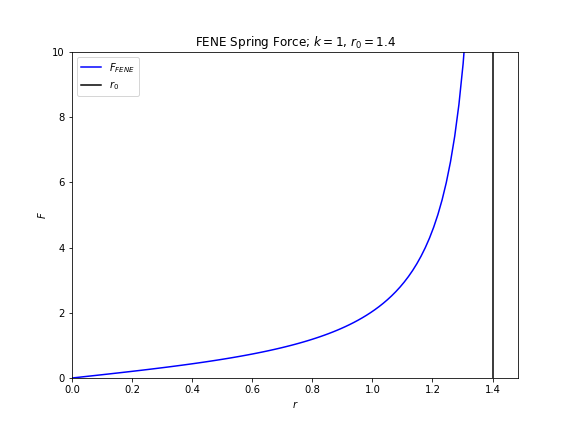
\includegraphics[height=4cm\textwidth]{./FENE.png}
\end{center}
\end{frame}

\begin{frame}[label={sec:org416f40e}]{The Model: Particles}
\begin{itemize}
\item Passive: Spherical
\item Active: Dumbbells formed by attaching spring between two spheres
\item Activity: Force with fixed magnitude acting on the two spheres of the dumbbell directed along the axis
\end{itemize}
\begin{figure}[htbp]
\centering
\includegraphics[height=2cm]{./Model.png}
\captionof{figure}{Diagram representing Active Dumbbell}
\end{figure}
\end{frame}

\begin{frame}[label={sec:org830f769}]{Equations of Motion: Langevin Dynamics}
\begin{itemize}
\item As particles are in a medium, either the particles in it or their effect on other particles need to be simulated
\item Langevin Dynamics allows us to simulate two key effects of the medium:
\begin{itemize}
\item Resistance to Movement i.e Viscosity; \(\propto \vb{v}(t)\)
\item Random force due to fluctuations in the medium's density: \(\xi(t)\)
\end{itemize}
\item Equations of Motion:
\end{itemize}
\begin{align*}
\dd{x_i}(t) &= v_i(t)\dd{t} \\
\dd{v_i}(t) &= m_i^{-1} F_i(x(t)) - \gamma_i v_i(t) \dd{t} + \sqrt{2 k_B T \gamma_i m_i^{-1}} \dd{W_i}(t)
\end{align*}
\end{frame}

\begin{frame}[label={sec:org296bbd3}]{Langevin Equations (Continued)}
\begin{itemize}
\item \(W(t)\) - Wiener Process
\begin{itemize}
\item \(W(0) = 0\)
\item Increments are independent: \(W(t+u) - W(t)\) is independent for all past values \(W(s)\) for all \(u, t > 0, s \leq t\);
\item Increments are from normal distribution: \(W(t+u) - W(t) \sim \mathcal{N}(0, u)\)
\item \(W\) is continuous in \(t\)
\end{itemize}
\begin{itemize}
\item Coefficient of last term derived from this condition
\begin{itemize}
\item \(\expval{v^2(t)}_{eq} = \frac{k_BT}{M}\)
\end{itemize}
\end{itemize}

\item Integration Scheme provided by: "Second-order integrators for Langevin equations with holonomic constraints" by E Vanden-Eijnden, G Ciccotti - Chemical physics letters, 2006. \href{https://doi.org/10.1016/j.cplett.2006.07.086}{https://www.sciencedirect.com/science/article/pii/S0009261406011092}
\item Modified Velocity Verlet Scheme
\end{itemize}
\end{frame}

\begin{frame}[label={sec:org28aa89b}]{Integrating Equations of Motion}
\begin{itemize}
\item Changing Notation: \(f_i(x) = m_i^{-1}F_i(x)\), \(\sigma = \sqrt{2 k_B T \gamma_i m_i^{-1}}\)
\end{itemize}
\begin{align*}
\dd{x_i}(t) &= v_i(t)\dd{t}\\
\dd{v_i}(t) &= f_i(x(t)) - \gamma_i v_i(t) \dd{t} + \sigma_i \dd{W_i}(t)
\end{align*}
\begin{align}
v^{n+1/2} ={}&v^n + \frac{1}{2} h f(x^n) - \frac{1}{2} h \gamma v^n + \frac{1}{2} \sqrt{h} \sigma \xi^n \notag\\
&-\frac{1}{8} h^2 \gamma \pqty{f(x^n) - \gamma v^n} - \frac{1}{4} h^{3/2} \gamma \sigma \pqty{\frac{1}{2} \xi^n + \frac{1}{\sqrt{3}} \eta^n} \\
x^{n+1} ={}&x^n + h v^{n+1/2} + \frac{1}{2\sqrt{3}}h^{3/2} \sigma \eta^n \\
v^{n+1} ={}&v^{n+1/2} + \frac{1}{2} h f(x^{n+1}) - \frac{1}{2} h \gamma v^{n+1/2} + \frac{1}{2} \sqrt{h} \sigma \xi^n \notag\\
&-\frac{1}{8} h^2 \gamma \pqty{f(x^{n+1}) - \gamma v^{n+1/2}} - \frac{1}{4} h^{3/2} \gamma \sigma \pqty{\frac{1}{2} \xi^n + \frac{1}{\sqrt{3}} \eta^n}
\end{align}

\begin{itemize}
\item Note that setting \(\gamma = \sigma = 0\) results in Velocity Verlet
\end{itemize}
\end{frame}

\begin{frame}[label={sec:org6c523a1}]{Implementation Details:}
\begin{block}{Algorithms Implemented:}
\begin{itemize}
\item Velocity Verlet
\item Optimization: Verlet Neighbour List
\item Thermostat: Langevin Equations
\item Potential: Truncated and Shifted Lennard-Jones Potential
\end{itemize}
\end{block}
\begin{block}{Code Details:}
\begin{itemize}
\item Language: Cython (C + Python)
\item Packages: NumPy + SciPy, matplotlib (for Plots and Animations)
\end{itemize}
\end{block}
\end{frame}

\begin{frame}[label={sec:org483aaa4}]{Testing Accuracy: Simulating LJ Fluid}
\begin{itemize}
\item Benchmark outlined by: "The Lennard-Jones equation of state revisited" by  JK Johnson, JA Zollweg, KE Gubbins - Molecular Physics, 1993. \href{https://www.tandfonline.com/doi/abs/10.1080/00268979300100411}{https://doi.org/10.1080/00268979300100411}
\item Involves simulating \(N=864\) particles with \(r_c = 4.0\sigma\) as the cutoff radius of LJ potential
\item Test Condition: Pass when potential energy within range given in paper
\item Benchmarked for only a few paramters: \(T^*=6\) with \(\rho^*\) ranging from 0.1 to 1.25
\item Future Plan: Benchmark using: "Efficient Computation of Entropy and Other Thermodynamic Properties for Two-Dimensional Systems Using Two-Phase Thermodynamic Model" by  SS Pannir Sivajothi, ST Lin, PK Maiti - The Journal of Physical Chemistry B, 2018. \href{https://pubs.acs.org/doi/10.1021/acs.jpcb.8b07147}{DOI: 10.1021/acs.jpcb.8b07147}
\end{itemize}
\end{frame}

\begin{frame}[label={sec:org96b9803}]{3D LJ Fluid Simulation}
\end{frame}


\begin{frame}[label={sec:org8dc81c6}]{Testing Accuracy: Langevin Dynamics}
\begin{itemize}
\item Simple test using relation between mean square displacement (MSD) vs Time for different parameters.
\end{itemize}
\begin{align*}
\expval{r^2(t)} = &v^2(0)\tau^2\pqty{1-e^{-t/\tau}}^2 + \frac{6k_BT}{m}\tau t\\
&- \frac{3k_BT}{m}\tau^2\pqty{1-e^{-t/\tau}}\pqty{3 - e^{-t/\tau}}
\end{align*}
where \(\tau = \gamma^{-1}\) is the relaxation time of the Brownian Motion
\begin{itemize}
\item Note that the above applies to 3D system where \(Nk_BT = 3K_BT\)
\item For small time scales: \(\expval{r^2(t\ll\tau)} = v^2(0)t^2\)
\item For large time scales: \(\expval{r^2(t\gg\tau)} = 6k_BT\tau t/m\)
\end{itemize}
\end{frame}

\begin{frame}[label={sec:org1653e6b}]{Testing Accuracy: Langevin Dynamics - Plots}
\begin{center}
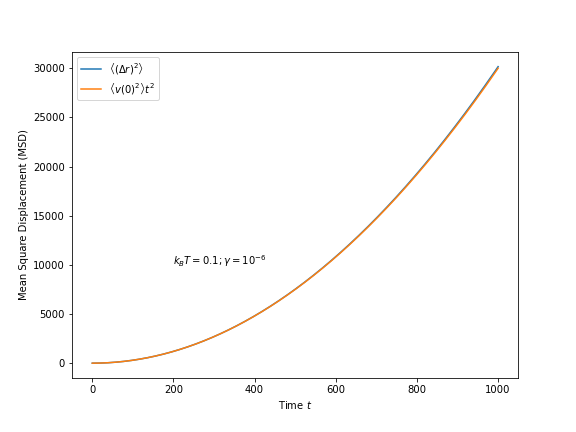
\includegraphics[height=4cm\textwidth]{./Lang1.png}
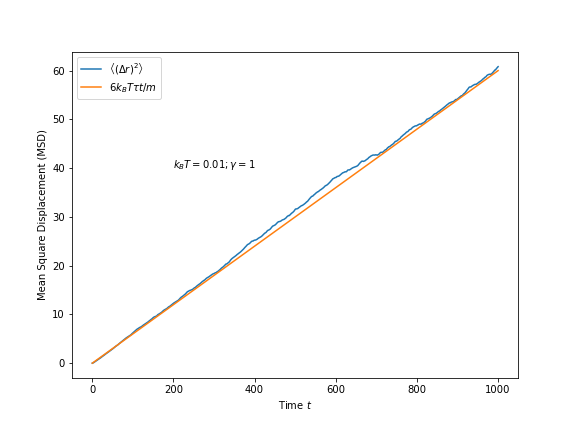
\includegraphics[height=4cm\textwidth]{./Lang2.png}
\end{center}
\end{frame}

\begin{frame}[label={sec:orgd52ab97}]{Simulating Active Particles: In Isolation}
\begin{center}
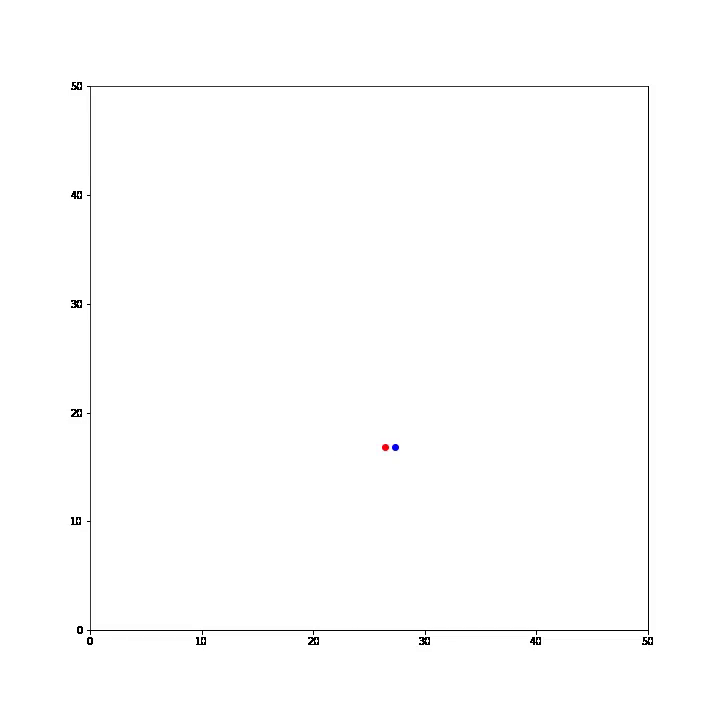
\includegraphics[height=7cm]{./Active1.png}
\end{center}

\href{./Active1.mp4}{Link to Video}
\end{frame}

\begin{frame}[label={sec:orgb54d356}]{Simulating Active Particles:}
\begin{figure}[htbp]
\centering
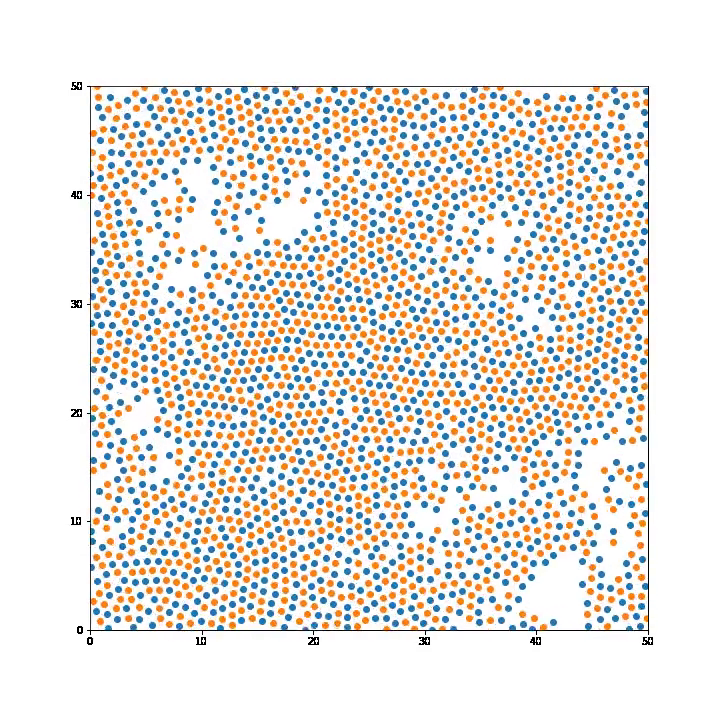
\includegraphics[width=6cm]{./Active3.png}
\captionof{figure}{Simulation of 2500 Active dumbbells in 50X50 Box; $F = 1$ and $T=0.001$}
\end{figure}

\href{./Active3.mp4}{Link to Video}
\end{frame}


\begin{frame}[label={sec:org71fcd63}]{Simulating Active Matter: Issues}
\begin{itemize}
\item To observe Phase Separation and internal flow, the number of particles required to simulate is very large, resulting in long calculation time and heavy memory requirements.
\item The code is single threaded.
\begin{itemize}
\item Multithreading via OpenMP is simple for NumPy (BLAS Operations), but needs to be explicit for Cython
\end{itemize}
\item Need to implement efficient algorithm for calculating LJ Interaction.
\end{itemize}
\end{frame}
\end{document}